% dynamic predication
%
\documentclass[10pt,twocolumn,dvips]{article}
%\documentclass[10pt,dvips]{article}
\usepackage[english]{babel}
\usepackage{epsfig}
\usepackage{rotating}
\usepackage{graphics}
%
%\usepackage{fancyheadings}
%\usepackage[T1]{fontenc}
%\usepackage[latin1]{inputenc}
%
%\usepackage{twocolumn}
%\usepackage{verbatim,moreverb,doublespace}
%\usepackage{rotate,lscape,dcolumn,array,rotating,latexsym}
%
%\input{epsf}
%
\textwidth 6.5in
\textheight 9.0in
\topmargin -0.6in
\oddsidemargin 0mm
\evensidemargin 0mm
%
%\pagestyle{empty}
%
\begin{document}
%\parskip 1mm
%
%
%
% continue with the rest of the paper
%
\title{Dynamic Predication and Fetch Heuristics}
%
%
\author{
A. Khalafi, D. Morano, D.R. Kaeli\\
Northeastern University\\
360 Huntington Ave.\\
Boston, MA. \\
{akhalafi, dmorano, kaeli}@ece.neu.edu \\
1 (781) 388-1799 \\
\and
A. Uht\\
University of Rhode Island\\
4 East Alumni Ave.\\
Kingston, RI.\\
uht@ele.uri.edu\\
1 (401) 874-5431
}
%
% no date
\date{}
%
%
\maketitle
%\thispagestyle{empty}
%
%
% add other front-matter here ?
\noindent{
contact author: Prof. David Kaeli \\
presentation author: Alireza Khalafi\\
keywords: predication dynamic fetch control-flow distributed
}
\vspace{-0.15in}
%
%
% abstract goes here if you have one
%
\begin{abstract}
Predicated execution of instructions is known to reduce control-flow
complications due to conditional branches.
Currently, either software-only or explicit architected 
instruction predication (for those architectures that have it)
has been employed.
However, software-only predication is very limited in its ability to
eliminate conditional branches from the instruction stream and
only new processor architectures have substantial support for
explicit architected predication. 
We introduce a hardware scheme that allows all instructions
to be predicated dynamically at execution time within the
microarchitecture of the machine.  This allows for
both legacy instruction set architectures to benefit from
instruction predication as well as opening up possibilities
for more advanced fetching heuristics in new microarchitectures.
Further, this scheme is oriented towards application to
distributed microarchitectures.

Our new instruction predication scheme builds on previous schemes
but avoids the complexity of them.
It also is more suitable for application to a distributed microarchitecture
than some previous schemes.
We also explore the effect of fetch policy on encountering conditional
branches.  Data is presented that shows substantial performance speedup.

\end{abstract}
%
%
\vspace{-0.25in}
\section{Introduction}
\vspace{-0.15in}
%
Explicit architectural predication has been of particular interest for
several years now.  Explicit architectural predication is implemented
through architecturally visible predicate registers as part of
an Instruction Set Architecture (ISA).  
An example of a popular
ISA that uses architected (or visible explicit) hardware predication 
is the {\it iA-64}
ISA family of machines~\cite{ia64}.

One hardware alternative to architected predication 
is to not
have any predicate registers defined in the ISA to start with
while still providing predication of instructions at the microarchitectural
level of the machine.
Instead predication is performed dynamically at program execution and is
referred to as simply {\it dynamic predication}.
One obvious advantage to this predication strategy is that it
can be applied to existing ISAs that never planned on using
any predication of any sort when they were first designed.  

Full microarchitectural based instruction predication
(dynamic predication that applies to all instructions in-flight)
is a new way to manage control dependencies that avoids added
complexity for recognizing special control-flow constructs.
With full microarchitectural predication
all conditional branches may execute concurrently 
and for those branch constructs with a join,
the code that lies
between the branch and its target instruction (the {\it domain} of the
branch ~\cite{Uht91}),
is now predicated and can be executed speculatively without additional
special
microarchitecture state that needs to be maintained for it.
Code that
lies beyond the joins of conditional branches is properly identified
as such (being control-independent of the branch)
and can be taken advantage of more easily (less hardware
complexity) than other approaches
such as that described by Cher et al ~\cite{Cher01}.

We are proposing a new dynamic predication scheme that can 
predicate all control-flow constructs rather than just
some specialized constructions.
Unlike other schemes, it features no centralized hardware resources,
thus making it very suitable for distributed microarchitectures.
Finally, the new scheme is simpler than all previously known
schemes in terms of hardware complexity.
%
\vspace{-0.25in}
\section{Background}
\vspace{-0.15in}
%
Several dynamic predication schemes are possible.
An early scheme described by Klauser et al ~\cite{klauser98dynamic}
applied dynamic predication to
hammock-styled conditional branch constructs only.
Further, it
was fairly complicated because it required the introduction
of a conditional micro-instruction operation
into the microarchitecture.  Other later schemes applied
predication to all control-flow constructs and did not require
such extensive additional micro-operations.

One later dynamic predication scheme that performed full
predication for all instructions
was described by Uht et al ~\cite{Uht02}.
Control-flow 
dependencies were evaluated to create predicates for each instruction
at dispatch time.
However, this scheme requires the
presence of a {\it Branch Tracking Buffer} that is used to correlate branch
target instructions with the original branch instructions that lead to
them.  
Unfortunately, the hardware needed to implement the tracking buffer
in order to search it for many dispatched instructions simultaneously
is very costly and does not scale well as the number of instructions
dispatched in a single clock grows.
Further, the presence of centralized tracking buffer introduces
signal routing and timing problems for large distributed microarchitectures.

Other dynamic predication schemes have been 
introduced ~\cite{Morano02,uht02levo}
that have eliminated the need for any centralized tracking buffer.
These newer schemes dynamically discover the control-flow dependencies
among instructions as they are in flight after instruction dispatch.
These newer schemes are especially suited to distributed microarchitectures
since they discover inter-instruction control-flow dependencies
in a distributed way.

The proposed scheme is oriented towards application on a distributed
microarchitecture ~\cite{Uht02,uht02levo} that uses time-tags for
dependency ordering of instructions and operands ~\cite{Kaeli01}.
Time-tags are small integers that provide and maintain the 
program order relationship among both instructions and operands.
Successive instructions are assigned successive time-tag values
and all operands that originate from instructions are tagged
with the time-tag value that was assigned to the instruction.
The instruction that is next to commit among all in-flight instructions
is assigned the lowest value (generally zero) and the most speculative
instruction will have the highest value.

Further, in those distributed microarchitectures that we are targeting,
the instruction issue window is spatially distributed in
silicon, having each issue slot potentially separated from the others.
Also, instructions stay in their issues slots that they were dispatched
to until either retirement, being either commitment or abandonment (squash).
Communication paths (buses) are available to propagate result operands 
(along with other associated information like its time-tag value) from
one instruction to the next.
%
%
\vspace{-0.25in}
\section{Dynamic Hardware Predication}
\label{sec:hwpred}
\vspace{-0.15in}
%
A principal requirement of the scheme is to generate
predicates as instruction execution proceeds.
Each instruction computes
its own enabling predicate using predicate values 
that are forwarded to it by earlier instructions from the
program-ordered past. 

\begin{figure}
%\vspace{0.2 in}
%\setlength{\epsfxsize}{10cm}%7
%\centerline{\epsfbox{window.eps}}
\centering
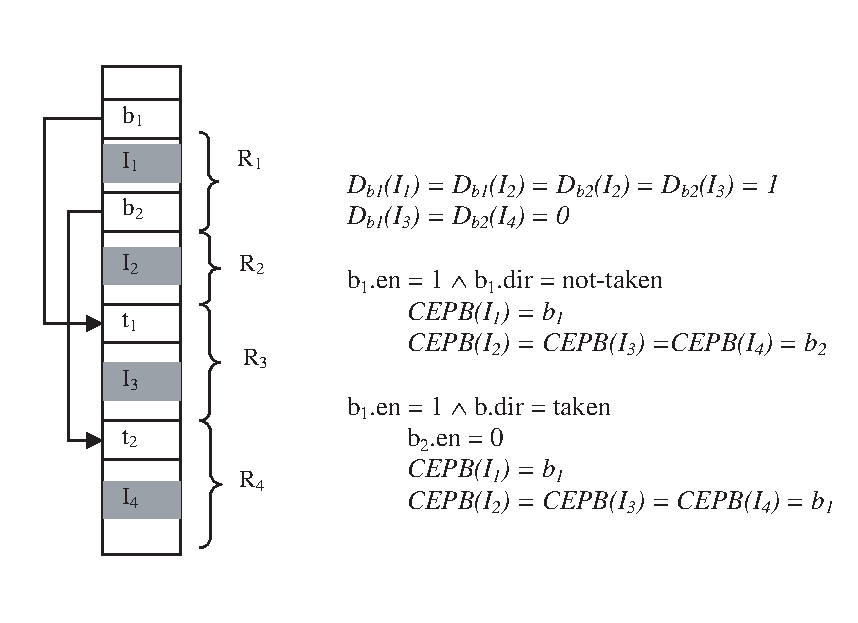
\epsfig{file=brdomain.eps,width=3.0in} \caption{Branch Domains and
Closest Enabled Previous Branch.(CEPB)} \label{fig:brdomain}
\end{figure}

Figure~\ref{fig:brdomain} shows a program code sequence with two
branches $b_1$ and $b_2$ and their corresponding targets $t_1$ and
$t_2$. The two branches divide the code into 4 basic blocks regions.
We are proposing a new scheme for
assigning an enabling predicate to every instruction in each
region based on the outcome of branches.  If the enabling
predicate value is one, then the instruction will be executed;
otherwise it is disabled.  The following definitions are used in
the description of our scheme.

%\begin{description}[\setlabelwidth{CEPB(Ij)xxx}]
\begin{description}{\setlength{\labelwidth}{3.0in}}
\item[$T_b$:] a binary value, set to one if the branch $b$ is predicted taken
\item[$en_j$:] a binary value assigned to each
instruction $I_j$ and specifies whether the instruction is
enabled for execution
\item[$D_b(I_j)$:] a binary value,
set to one if the instructions $I_j$ is in the domain of branch $b$.
\item[$CEPB(I_j)$:] Closest Enabled Previous Branch to instruction
$I_j$ in the static program-order.
\end{description}

In Figure~\ref{fig:brdomain} we have also shown the value of CEPB and $D_b$ variables
for the two branches in the figure.
The $D_b(I)$ function is
independent of the outcome of the branch and only depends on the
static order of the instructions in the code.  $CEPB(I)$, on the other
hand, is a function of the outcome of other branches and its value can
change during the course of speculative execution.

Using the above definitions, we can show that:
\begin{equation}
\overline{en_j} = T_b \cdot D_b(I_j)  \textstyle{\ where\ } b = CEPB(I_j)
\label{eq:preden}
\end{equation}

This equation simply tells us that if an instruction $I_j$ is in
the domain of an enabled branch, and if the branch is taken, $I_j$ will
not be executed.  If the instruction is out of the domain of its closet
enabled previous branch, then its execution is independent of the
outcome of the branch.
Equation~\ref{eq:preden} is the basis for our dynamic predication scheme.

To assign a predicate value to each instruction $I_j$, it is sufficient
to find the $CEPB(I_j)$ branch and its outcome.  This is a simple
task in our scheme.  Each instruction in an issue slot
has a pair of
registers to keep the time-tag of its current $CEPB$ branch and
branch target.

If an earlier branch is enabled, a transaction is sent on the
forwarding bus with the branch time-tag, its target address and whether
it is a taken branch or not. 
Each subsequent instruction that snoops
this transaction checks to see if the time-tag of the newly enabled
branch is greater than the time-tag of its current CEPB branch.  If the
time-tag of the new branch is greater, the new branch must be closer to
this instruction, and therefore it will replace the older $CEPB$
branch.

If a branch $b$ becomes disabled, the later instructions need to find
another branch to act as their new $CEPB$ branch.  This new branch is
simply $CEPB(b)$, because according to the definition there is no other
enabled branch between $CEPB(b)$ and $b$. In our scheme this is
achieved  by initiating an invalidate transaction at branch $b$. An
invalidate transaction contains the time-tag of $b$, the time-tag of
$CEPB(b)$ and the branch domain information of $CEPB(b)$.  This
information was snooped by $b$ when $CEPB(b)$ forwarded its predicate.

To find the domain of a $CEPB$ branch, a simple approach is to just
compare the branch target address with the instruction address.
It is however more efficient to use time-tags for this purpose.
A branch only needs to forward the time-tag of its target
instruction instead of its target address. The branch target
time-tag can be easily calculated by adding the branch
displacement to the branch time-tag value.

Another improvement to the above scheme can be made by observing
that a not-taken enabled branch does not need to send out any
transaction on the forwarding bus.  This is due to the fact that a
not-taken branch essentially acts like a NOP operation.  We can take
advantage of this knowledge by reducing the number of transactions on the
communicating bus.

\begin{figure}
%\vspace{0.2 in}
%\setlength{\epsfxsize}{10cm}%7
%\centerline{\epsfbox{window.eps}}
\centering
\epsfig{file=dynpred.eps,width=3.0in} \caption{Example illustrating
Dynamic Predication} \label{fig:dynpred}
\end{figure}

Figure~\ref{fig:dynpred} shows an example of how our dynamic
predication work.  The first column in the table lists the relative
clock cycles.  The next three columns list the status of each
branch.  The "D", "T' and "NT" entries correspond to disabled,
taken and not-taken status, respectively.  The next two columns
list the status of instruction $I_k$.  The labels "E" and "D" stand for enabled
and disabled status, respectively.  The $CEPB$ column shows the
$CEPB(I_k)$ branch at any cycle.  The next two columns show the
transactions on the bus.  The "PredVal" column lists the predicate
forwarding transactions for each branch along with its status.  The
"PredInv" column lists the invalidating transactions.  the branch
name in the parenthesis corresponds to the new $CEPB$ forwarded by
the invalidated branch.

In the example, it is assumed that $b_1$ and $b_3$ are initially
predicted taken and not-taken respectively.  As a result,
instruction $I_k$�s predicate is enabled.  In the next
cycle, $b_1$ changes its direction to
not-taken and sends a forwarding transaction on the bus
indicating this change.
This transaction will enable $b_2$ which is also predicted taken.
Branch $b_2$ will send a predication transaction on the forwarding bus
which is snooped by $b_3$.  As a result, $b_3$ will be disabled in
cycle 3 and will send an invalidating transaction with $b_2$ as
its $CEPB$ branch.  instruction $I_k$ will see this transaction and
switch its $CEPB$ to $b_2$ and will be disabled.  The
second part of the table in figure~\ref{fig:dynpred} shows what
will happen if $b_1$ changes back to a taken status.  A new set of
transactions will follow that eventually enable $I_k$.
The cost of hardware predication is low and most of the extra state
only uses a few bits in the issue slot.  
%
\vspace{-0.25in}
\section{Fetch Heuristics}
\vspace{-0.15in}
%
A set of heuristics are developed to guide I-fetch and take
advantage of dynamic predication. In the case of forward branches,
we define two threshold values: \emph{near} and \emph{far}. We
then compare the branch domain size with the threshold values to
categorize a branch as \emph{near} (less than the near value),
\emph{moderate} (between near and far) or \emph{far} (greater than
the far value). Since the domain of a forward branch possessing a
near target is small and can be easily fit within the execution
window, the fetch unit will load the instructions following the
not-taken path of the branch, regardless of its prediction.
Fetching and loading instructions following the not-taken path of
a conditional branch will capture hammock-styled branch
constructs. 

For a conditional branch with a moderate-distance target (neither
near nor far), we use a confidence predictor~\cite{jacobsen96assigning}
to measure the accuracy of the branch
predictor. If the branch can be predicted with high confidence,
the instructions are fetched from the predicted path, otherwise
fetch continues from the sequential instructions after the branch.
By fetching the domain of the branch, in case the branch is
mispredicted, there is no need to flush the execution window. 

In case of a conditional branch with a far target, we will always
follow the predicted path to avoid loading a large number of useless
instructions into the execution window.

If a conditional backward branch is predicted taken, it will be treated
as a loop, and fetch/dispatch will follow the taken path of the branch.
This policy will basically unroll the loop and fill the execution
window with successive iterations of the loop.
%
\vspace{-0.25in}
\section{Results}
\vspace{-0.15in}
%
We evaluated the effect of choosing different values for \emph{near}
and \emph{far} branch thresholds using a set of benchmarks form Spec95
and Spec2000\footnote{Spec95: go, compress, ijpeg; Spec2000: bzip2,
crafty, gcc, gzip, mcf, parser, vortex}.  Table~\ref{tab:results} 
shows the harmonic mean of percent
speedup over all benchmarks as a function of conditional branche 
threshold value.
In our base configuration instructions
are always fetched from the predicted path.  The results 
in Table~\ref{tab:results} 
show that for a fixed \emph{far} threshold, as 
we increase the \emph{near}
threshold, the speedup increases.  For near threshold values
greater than 16, the speedup starts to decrease.  The reason 
for this performance degradation is that we
are fetching more and more branches from the fall-through path
regardless of their prediction.  This means a higher ratio of
dispatched instructions are squashed at commit time which results
in performance loss.

\begin{table}
\begin{center}
\caption{Relative harmonic mean (as a percent) performance as a function of
conditional branch target distance thresholds. (FT: Far Threshold)}
\label{tab:results}
\begin{tabular}{|l|c|c|c|c|c|c|c|}
\hline 
&\multicolumn{7}{c|}{Near Threshold}\\
\hline
FT&1&2&4&8&16&32&64\\
\hline
1&0.0&&&&&&\\
2&0.0&0.0&&&&&\\
4&-0.8&-0.8&0.6&&&&\\
8&-1.5&-1.5&-1.2&3.6&&&\\
16&-2.7&-2.7&-2.3&2.7&3.4&&\\
32&-3.3&-3.3&-3.0&1.9&2.8&1.1&\\
64&-3.3&-3.3&-3.0&1.8&2.8&1.1&-0.7\\
\hline
\end{tabular}
\end{center}
\end{table}

Another observation in Table~\ref{tab:results} is that for a 
fixed near threshold, 
increasing the far threshold value reduces speedup and in many cases 
produces a slowdown.
These results indicate that using a confidence predictor
to handle moderate branches does not perform as well as fetching
from the branch fall-through path.
One explanation for this is that
relying on the confidence predictor alone does not consider the
merit of fetching from the fall-through branch path.
Fetching from fall-through and predicating those instructions 
is still advantageous for highly predictable 
branches, since it avoids the discontinuity of following the 
target of the branch.
Our results show that 
for our dynamic predication scheme to achieve its highest performance,
using a confidence estimator is not necessary.

From the table it can be seen that maximum performance is achieved 
when both \emph{far} and \emph{near} thresholds are the same.
In effect this means that only one threshold is necessary 
for guiding fetch beyond the branch.  
Over all benchmarks, 
using predication we achieved an average speedup of 3.6\% 
over our baseline machine.  This speed up was achieved using a value 
of 8 for both \emph{near} and \emph{far} threshold values.  
%
%
\vspace{-0.25in}
\section{Conclusions}
\vspace{-0.15in}
%
We have introduced a new scheme for the full execution-time
predication of all instructions within the microarchitecture
(dynamic predication).
This scheme not only allows for applicability to legacy ISAs
but avoids implementation difficulties with centralized 
hardware resources and is thus suitable for new distributed
microarchitectures. 
It is also simpler than all previous
dynamic predication schemes.
The data presented showed that using just one static 
threshold for determining fetch direction following a conditional
branch achieves best performance.
%
%
%
\bibliographystyle{latex8}
\bibliography{pdpta}
\end{document}
%
%
